计算机硬件主要由\textbf{存储器、运算器、控制器、输入设备和输出设备}组成({输入/输出设备统{称I/O设备}}),它们之间的关系如图1-1所示。

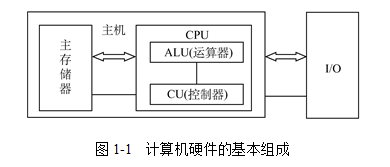
\includegraphics[width=3.70833in,height=1.58333in]{png-jpeg-pics/F1D18B7B5F3613863EFB8F429BC35B5B.png}

\textbf{其中,运算器+控制器=CPU,CPU+主存储器=主机,I/O设备又称为外部设备。}

\textbf{主存储器(主存):}存放程序和数据的部件。它是计算机实现``存储程序控制''的基础。

\textbf{运算器:}对信息进行处理和运算的部件,经常进行算术和逻辑运算,其核心是算术逻辑单元(ALU)。

\textbf{控制器:}是整个计算机的``指挥中心'',它使计算机各个部件自动协调工作。计算机中有两种信息在流动:一种是控制信息;另一种是数据信息。

\textbf{输入设备:}将人们所熟悉的信息形式转换成计算机可以接收并识别的信息形式的设备,例如键盘,当按下一个键时,此键被翻译成ASCII码传输给计算机,而ASCII码就是计算机可以接收并识别的信息形式。

\textbf{输出设备:}可将二进制信息转换成人类或其他设备可以接收或识别的信息,如显示器。
